\subsubsection{Malaclemys --- Diamondback Terrapins}
\begin{center}
\begin{longtabu} to \textwidth {| | p{3.5cm} | X | |}

	\hline
	Taxonomy/Ancestry &
	a member of the Deirochelyinae subfamily. a monotypic genus containing only the \emph{M. terrapin} species, w/ 7 subspecies recognized.
	
	\begin{center} \includegraphics[scale=0.5]{testudines/emydidae/malaclemys/tax} \end{center}
	 \\
	\hline
	Size & 
	males --- 13 cm (5.1) in; 300 g (11 oz). sexually mature at 2-3 yrs and 4-5 in of length
	
	females --- 19 cm (7.5 in); 300 g (11 oz). sexually mature at 6-7 yrs and 6.75 in of length
	\\
	\hline
	Color &
	named for the diamond patterned growth rings on carapace. unique patterns of wiggly black markings/spots on the body and head.
	 \\
	\hline
	Anatomy &
	\begin{itemize}[noitemsep]
		\item wedge-shaped shell wider from back than front
		\item large webbed feet
		\item species from warmer regions are larger
		\item adapted to marine environment near the shore
			\begin{itemize}[noitemsep]
				\item impermeable skin can stay in salt water for extended periods of time
				\item lachrymal salt glands
				\item can distinguish b/w drinking water of different salinities
				\item behavior to obtain freshwater --- drink freshwater surface layer on top of salt water during rainfall; raising head to catch rain drops
			\end{itemize}
	\end{itemize}
	 \\
	\hline
	Dimorphism & 
	females larger than males.
	\\
	\hline
	Behavior & 
	the behavior of \emph{Malaclemys} is mostly unknown due to their aquatic nature. it is suggested that nesting is the only activity that they perform on land. they most likely hibernate during colder months.
	\\
	\hline
	Habitat & 
	\begin{itemize}[noitemsep]
		\item coastal habitats --- estuaries, tidal creeks, salt marshes
		\item typically cordgrass marshes that flood at high tide, but also live in mangrove swamps in Florida
		\item survive in both freshwater and ocean water but prefer intermediate salinities
		\item no long-distance migrations
	\end{itemize}
	\\
	\hline
	Distribution & 
	narrow strip of coastal habitats on Atlantic and Gulf coasts of US --- Cape Cod to southern tip of Florida and around Gulf Coast to Texas
	\\
	\hline
	Feeding Ecology & 
	shrimps, clams, mussels, and other marine invertebrates, especially periwinkle snails.
	\\
	\hline
	Reproductive Biology & 
	see Emydidae entry for courtship and mating.
	
	\begin{itemize}[noitemsep]
		\item females wander considerable distances before nesting
		\item nest in sand dunes or scrub vegetation near ocean in June or July
		\item clutch sizes vary latitudinally ? 5.8 in S. Florida to 10.9 in NY
		\item after covering nest, female returns to ocean and does not come back to nest
		\item usually hatch in 60-85 days in August/September. the hatchlings, which are freeze-tolerant but have a lower salt tolerance, may overwinter in the nest.
		\item exhibit TSD --- warmer temperatures produce females, cooler temperatures produce males
	\end{itemize}
	\\
	\hline
	Ecological Role &
	at high densities, may eat enough invertebrates to significantly impact ecosystem, especially b/c periwinkles can overgraze important marsh plants
	\\
	\hline
	Conservation Status & 
	\begin{itemize}[noitemsep]
		\item Classified NT due to decreasing pop. \#s within range
		\item Limited protection on state-by-state level
		\item 1900s --- considered delicacy to eat, almost hunted to extinction
		\item Severely depleted by land development along Atlantic coast
		\item Receive wounds from propellors on motorboats
		\item Get trapped in crabbing/lobster nets
	\end{itemize}
	\\
	\hline
\end{longtabu}
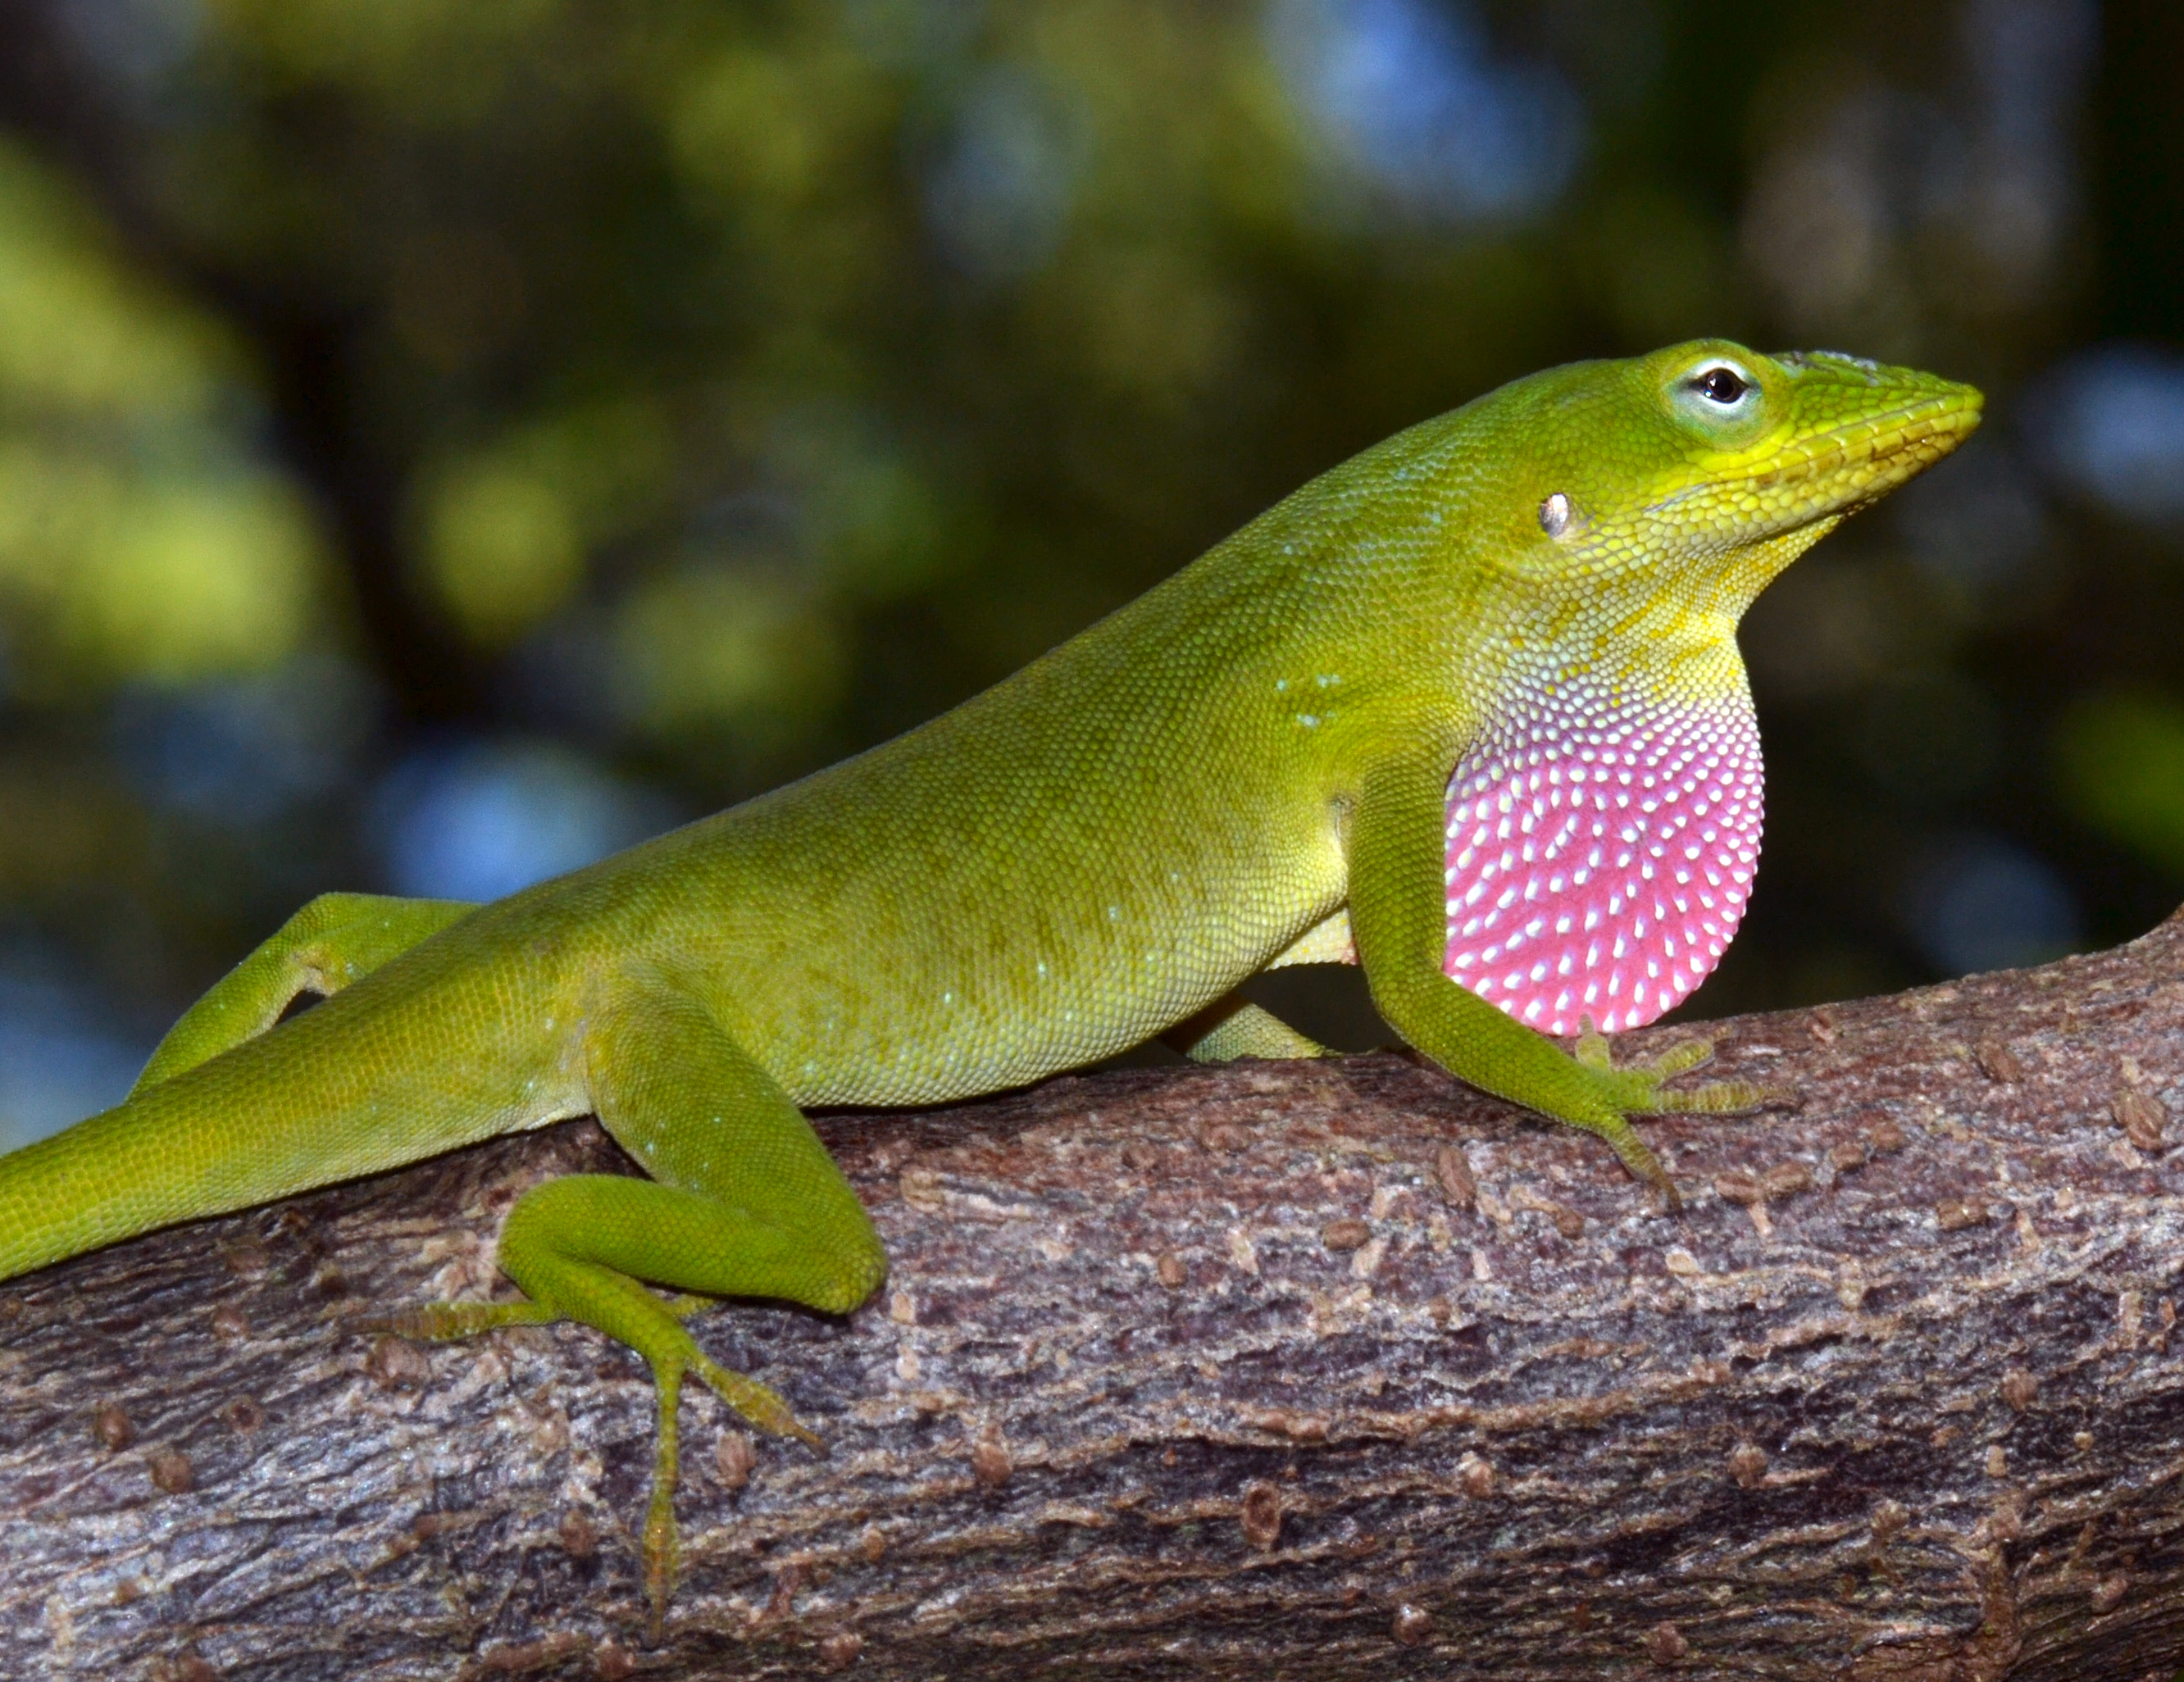
\includegraphics[scale=0.075]{testudines/emydidae/malaclemys/1}
\includegraphics{testudines/emydidae/malaclemys/2}
\end{center}